\documentclass[aspectratio=169,xcolor={dvipsnames}]{beamer}
\mode<presentation> {

\usetheme{Boadilla}

\usecolortheme{rose}


\definecolor{cardinal}{RGB}{140,21,21}

\setbeamertemplate{itemize items}[default]
\setbeamertemplate{enumerate items}[default]
\setbeamertemplate{section in toc}{\hspace{0.5cm}\large{\inserttocsectionnumber.~\inserttocsection}}
\setbeamertemplate{subsection in toc}{%
  \hspace{1.2em}\normalfont{\inserttocsubsectionnumber.~\inserttocsubsection\par}}

\setbeamercolor{structure}{bg=black, fg=cardinal}
\setbeamercolor{alerted text}{fg=cardinal}
\setbeamercolor{block body}{fg=black, bg=cardinal!10}
\setbeamercolor{block title}{fg=cardinal, bg=cardinal!10}
% \AtBeginSection{\frame{\sectionpage}}
% \AtBeginSubsection{\frame{\subsectionpage}}

\setbeamertemplate{footline}{}
\setbeamertemplate{blocks}[rounded][shadow=false]

\setbeamertemplate{navigation symbols}{} % To remove the navigation symbols from the bottom of all slides uncomment this line
}
% \usepackage{xcolor}
% \usepackage{tikz}
\usepackage{soul}
\usepackage{graphicx}
\graphicspath{{../../results/apr4th/images/}}
% \usepackage{booktabs}
% \usepackage{biblatex}
% \bibliography{ref.bib}
\usepackage{tabularx}
\usepackage{multirow}
\usepackage{hhline}
\usepackage{amsmath}
\usepackage{appendixnumberbeamer}


% \NeedsTeXFormat{LaTeX2e}
% \ProvidesPackage{nomenclature}[Nomenclature package]

\usepackage{ar}
\newcommand{\cldat}{\boldsymbol{{c_l}^{2D}}}
\newcommand{\CDp}{C_{D_p}}
\newcommand{\CDi}{C_{D_i}}
\newcommand{\cl}[1]{{c_l}_{\bf #1}}
\newcommand{\cdp}[1]{{c_{d_p}}_{\bf #1}}
\newcommand{\cb}[1]{\left(
	\frac c b 
\right)_{#1}
}
\newcommand{\An}[1]{\bar{A{#1}}}
\newcommand{\cddat}{\boldsymbol{{c_{d_p}}^{2D}}}

\title[Maximum Lift to Drag Ratio Glider Optimization]
{\huge{\textbf{Maximum Lift to Drag Ratio Glider Optimization}}} % The short title appears at the bottom of every slide, the full title is only on the title page
\author{Jean de Becdelièvre}

\begin{document}
\newcolumntype{C}[1]{>{\centering\arraybackslash}p{#1}}
\newcolumntype{L}[1]{>{\arraybackslash}p{#1}}

%%%%%%%%%%%%%%%%%%%%%%%%%%%%%%%%%%%%%%%%
% TITLE
%%%%%%%%%%%%%%%%%%%%%%%%%%%%%%%%%%%%%%%%
\begin{frame}
	\titlepage
\end{frame}

\begin{frame}
	Since last week:
	\begin{itemize}
		\item Consolidated optimization
		\item Ran test cases for simple 2D section models (flat plate, ...)
		\item Ran a full sweep on aircraft weight and tried to understand results
	\end{itemize}
	\tableofcontents
\end{frame}

 %% -------------------------- %%
\section{Optimization Problem}
\begin{frame}
	 \frametitle{Optimizing Glider L/D}
	 \begin{itemize}
		\setlength{\itemsep}{0pt}
		\setlength{\parskip}{0pt}
			 \item Maximizing gliding distance
			 \item Fixed weight W
			 \item Fixed airfoil section, known function $\cddat(Re, c_l)$ 
			 for  $c_l \in [\cl{lb}, \cl{ub}]$   and $Re \in [{Re}_{\bf lb}, {Re}_{\bf ub}]$ 

			\begin{align*}
				& \underset{}{\text{minimize}} & & C_D / C_L &  \\
				& \text{subject to} 
				& & C_L^2 + C_D^2 = C_W^2 \\
				& & & \cl{lb} \leq \cl{k} \leq \cl{ub}\\
				& & & {Re}_{\bf lb} \leq {Re}_{\bf k} \leq {Re}_{\bf ub}\\
			\end{align*}
			\end{itemize}
\end{frame}
% %% -------------------------- %% 


 %% -------------------------- %%
\begin{frame}
	 \frametitle{Reformulated Objective Function}
% 	 \begin{columns} 
% 		\begin{column}{0.5\textwidth}
% 			3 groups of design variables:
% 			\begin{enumerate}
% 			\setlength{\itemsep}{0pt}
% 			\setlength{\parskip}{0pt}
% 				  \item $Vb$
% 				  \item $\frac{c_1}{b}, \frac{c_2}{b}, \dots, \frac{c_{N_{y}/2}}{b}$ 
% 				 \item  $A_3/A_1, A_5/A_1, \dots A_{N_a}/A_1$
% 			\end{enumerate}
% 		\end{column}

% 		\begin{column}{0.5\textwidth}
% 			1 parameter: W
% 		\end{column}
%    \end{columns}

   \begin{align*}
	& \underset{Vb, \cb{1:N_y}, \An{2:N_a}}{\text{minimize}}  &
	\frac{4W}{\pi \rho^2 (Vb)^2} \left(1+\sum_{n=2}^{N_a} n \An{n}^2\right) &+
(Vb)^2 \sum_{k=0}^{N_y} w_k \cb{k} \cddat(\cl{k}, Re_k) & \\
	& \text{subject to} & \cl{lb} \leq &\cl \leq \cl{ub} \\
	& & {Re}_{\bf lb} \leq &{Re} \leq {Re}_{\bf ub} 
\end{align*}

with:
$$Re_{k} = \frac{\rho}{\nu}\cb{k}(Vb) $$

$$
	\cl{k} = \frac{8W}{\pi \rho (Vb)^2\cb{k}} \left(\sin(\theta_k) + \sum_{n=2}^{N_a} \An{n} \sin(n \theta_k)\right)
$$
\end{frame}
%% -------------------------- %% 


 % -------------------------- %%
\section{Sweep on W}
\begin{frame}
	 \frametitle{Sweep on W: $L_D$ and $\AR$}
	 \begin{columns} 
 
		  \begin{column}{0.5\textwidth}
			\begin{figure}
				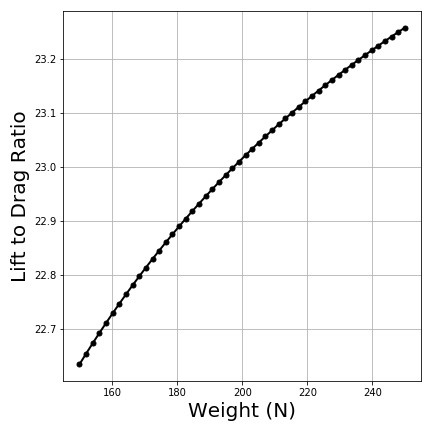
\includegraphics[width=0.8\textwidth]{L_D.png}
				\raggedleft
		   \end{figure}
		  \end{column}

		  \begin{column}{0.5\textwidth}
			   \begin{figure}
					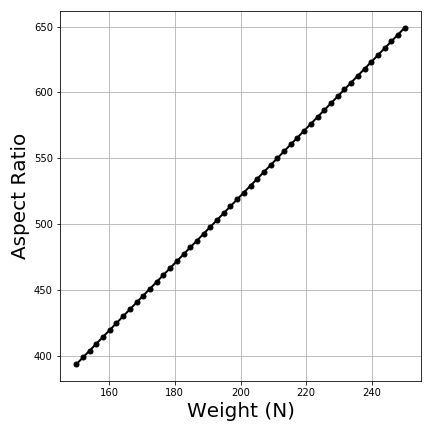
\includegraphics[width=0.8\textwidth]{AR}
					\raggedright
			   \end{figure}
		  \end{column}

	 \end{columns}
\end{frame}

\begin{frame}
	\frametitle{Sweep on W: $Re$ and $C_L$}
	\begin{columns} 

		 \begin{column}{0.5\textwidth}
		   \begin{figure}
			   \includegraphics[width=0.8\textwidth]{Re.png}
			   \raggedleft
		  \end{figure}
		 \end{column}

		 \begin{column}{0.5\textwidth}
			  \begin{figure}
				   \includegraphics[width=0.8\textwidth]{CL}
				   \raggedright
			  \end{figure}
		 \end{column}

	\end{columns}
\end{frame}
%% -------------------------- %% 

\begin{frame}
	\frametitle{Sweep on W: $\CDi$ and $\CDp$}
	Note the difference in scale.
	\begin{columns} 

		 \begin{column}{0.5\textwidth}
		   \begin{figure}
			   \includegraphics[width=0.8\textwidth]{CDi.png}
			   \raggedleft
		  \end{figure}
		 \end{column}

		 \begin{column}{0.5\textwidth}
			  \begin{figure}
				   \includegraphics[width=0.8\textwidth]{CDp}
				   \raggedright
			  \end{figure}
		 \end{column}

	\end{columns}
\end{frame}
%% -------------------------- %% 
			
\begin{frame}
	\frametitle{Sweep on W: planform shape}
	\begin{figure}
		\includegraphics[width=0.8\textwidth]{c_b}
		\centering
	\end{figure}
\end{frame}

\begin{frame}
	\frametitle{Sweep on W: lift distribution $\frac{c_l c}{c_L S/b}$}
	\begin{figure}
		\includegraphics[width=0.8\textwidth]{lift}
		\centering
	\end{figure}
\end{frame}


\end{document}